
\begin{frame}{Logistic Regression package}

\begin{columns}[T]
\vspace*{1em}\begin{column}{0.5\textwidth}
\lstinline|alpha = 1   \# Lasso = 1 -- Ridge = 0 -- 0 < Elastic < 1|
\lstinline|cv.model = cv.glmnet(x.train, y.train, family="binomial", alpha=alpha)|
\lstinline|best.lambda <- cv.model$lambda.min|
\end{column}
\begin{column}{0.5\textwidth}
\hspace*{-1em}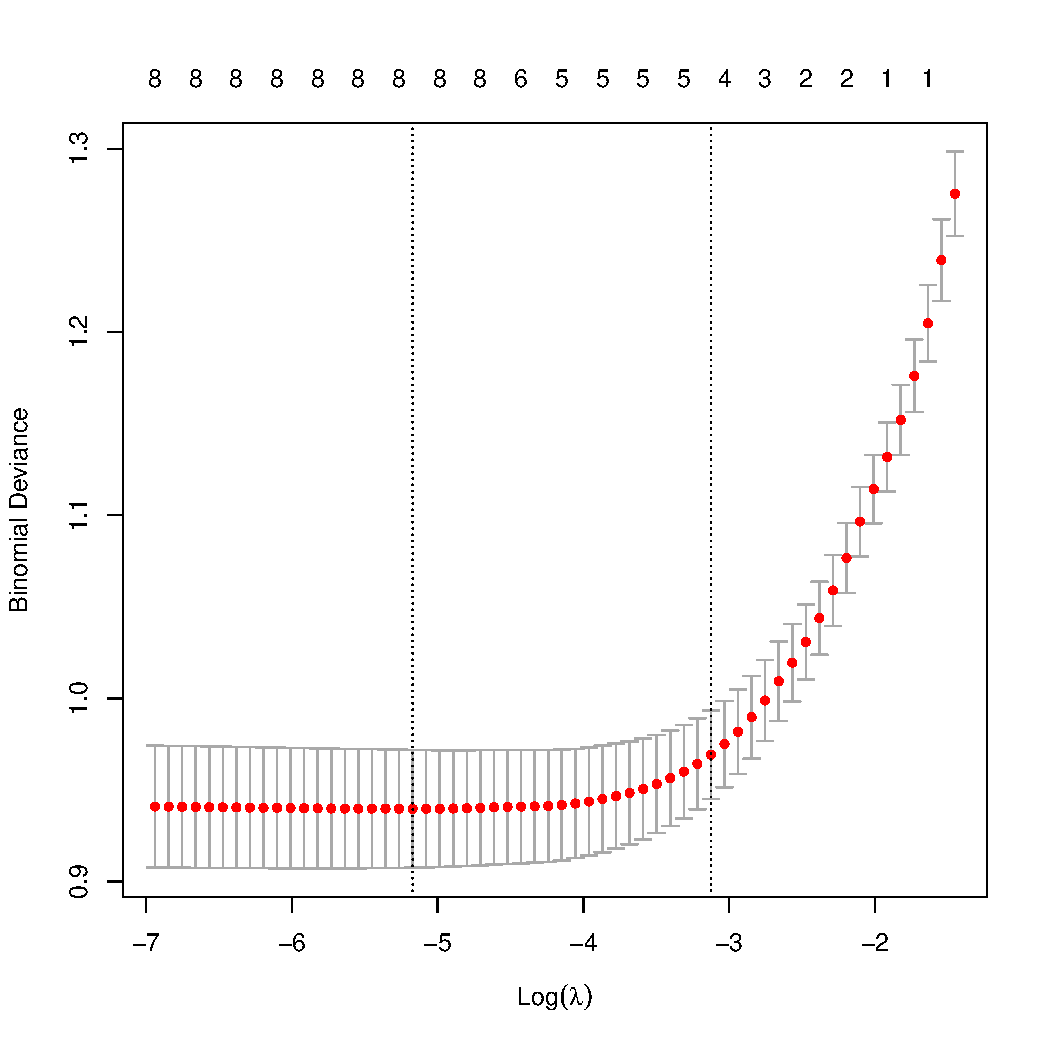
\includegraphics[width=1.2\columnwidth]{./Figures/logist/cv_lambda.pdf}
\end{column}
\end{columns}

\end{frame}

\begin{frame}{Ridge and Lasso variable importance}

\vspace*{-1em}\begin{columns}[T]
\begin{column}{0.5\textwidth}
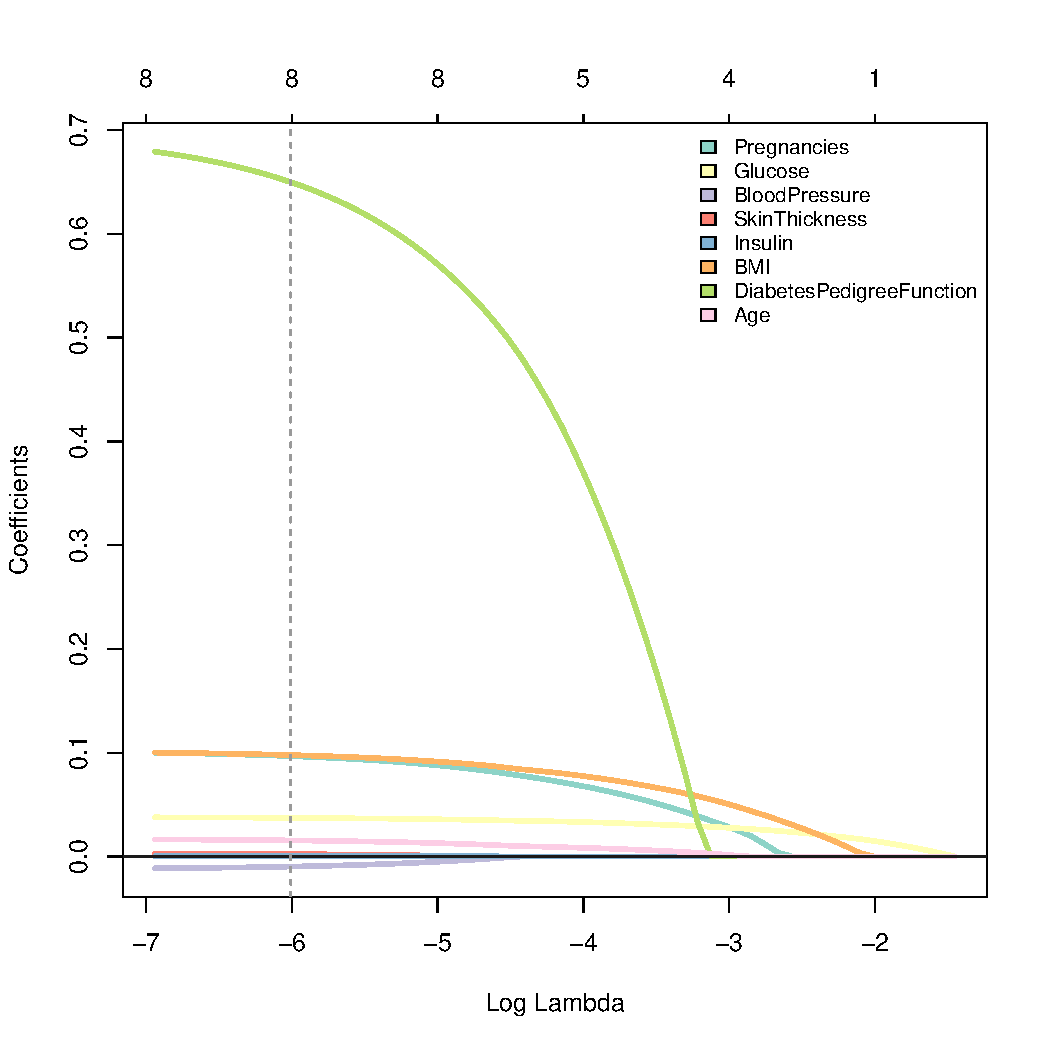
\includegraphics[width=0.85\columnwidth]{./Figures/logist/diabetes_lasso.pdf}
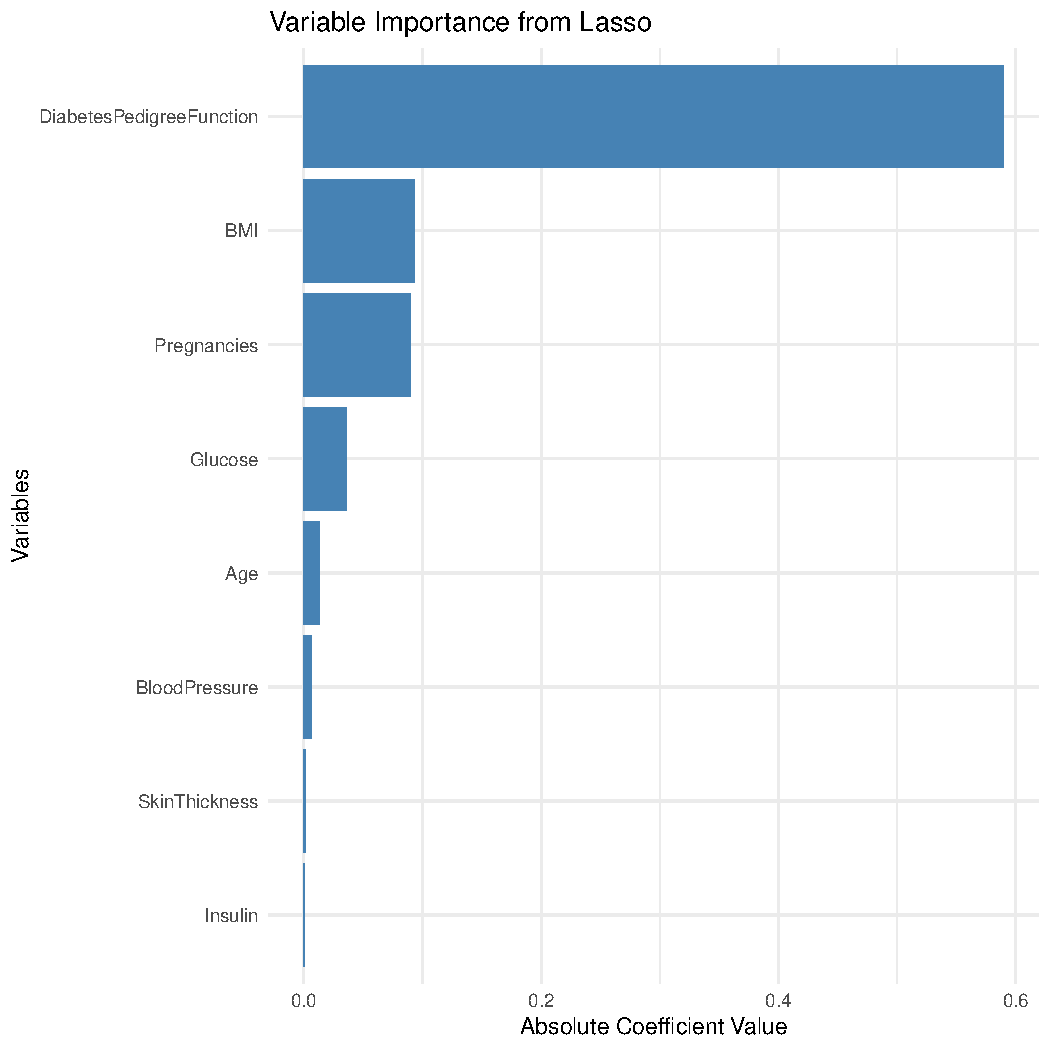
\includegraphics[width=0.7\columnwidth]{./Figures/logist/variable_importance_lasso.pdf}
\end{column}
\begin{column}{0.5\textwidth}
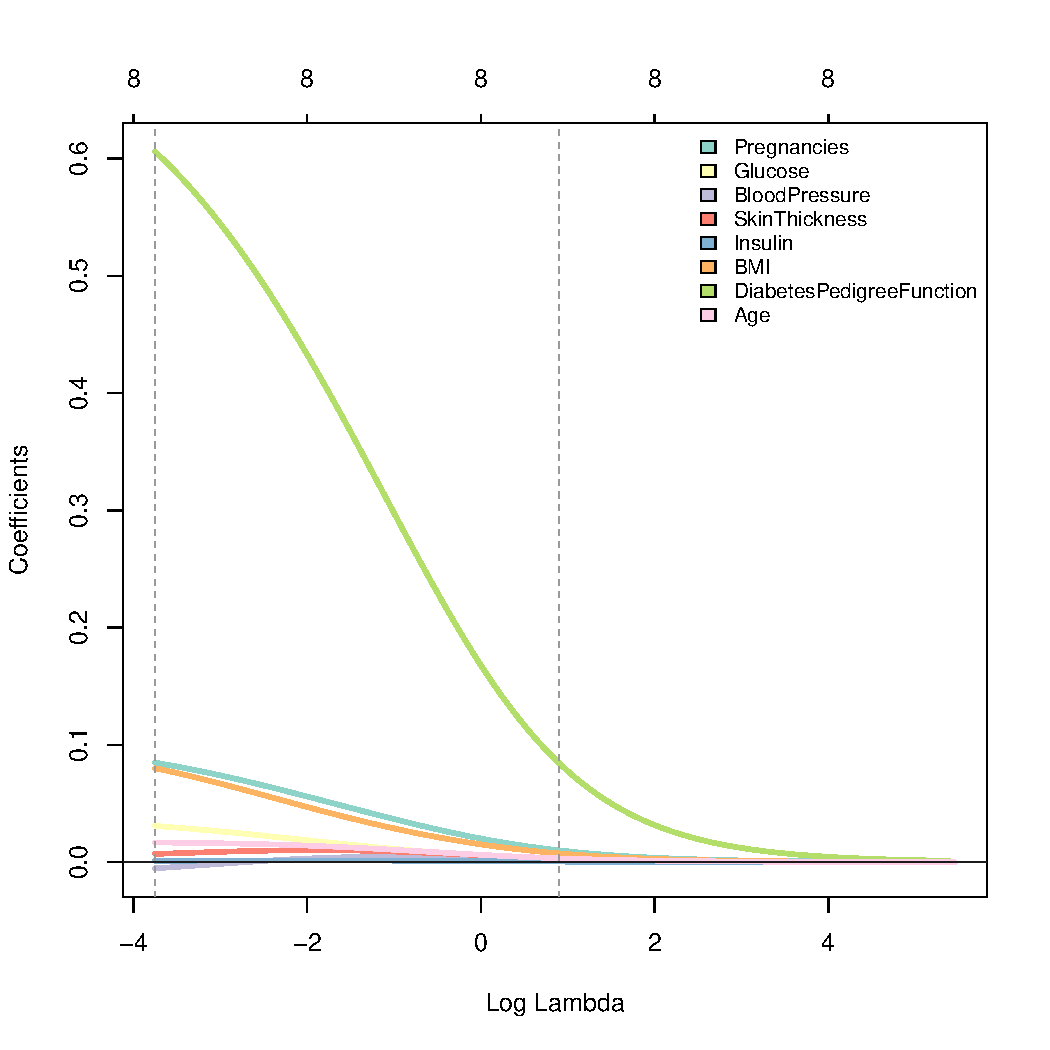
\includegraphics[width=0.85\columnwidth]{./Figures/logist/diabetes_ridge.pdf}
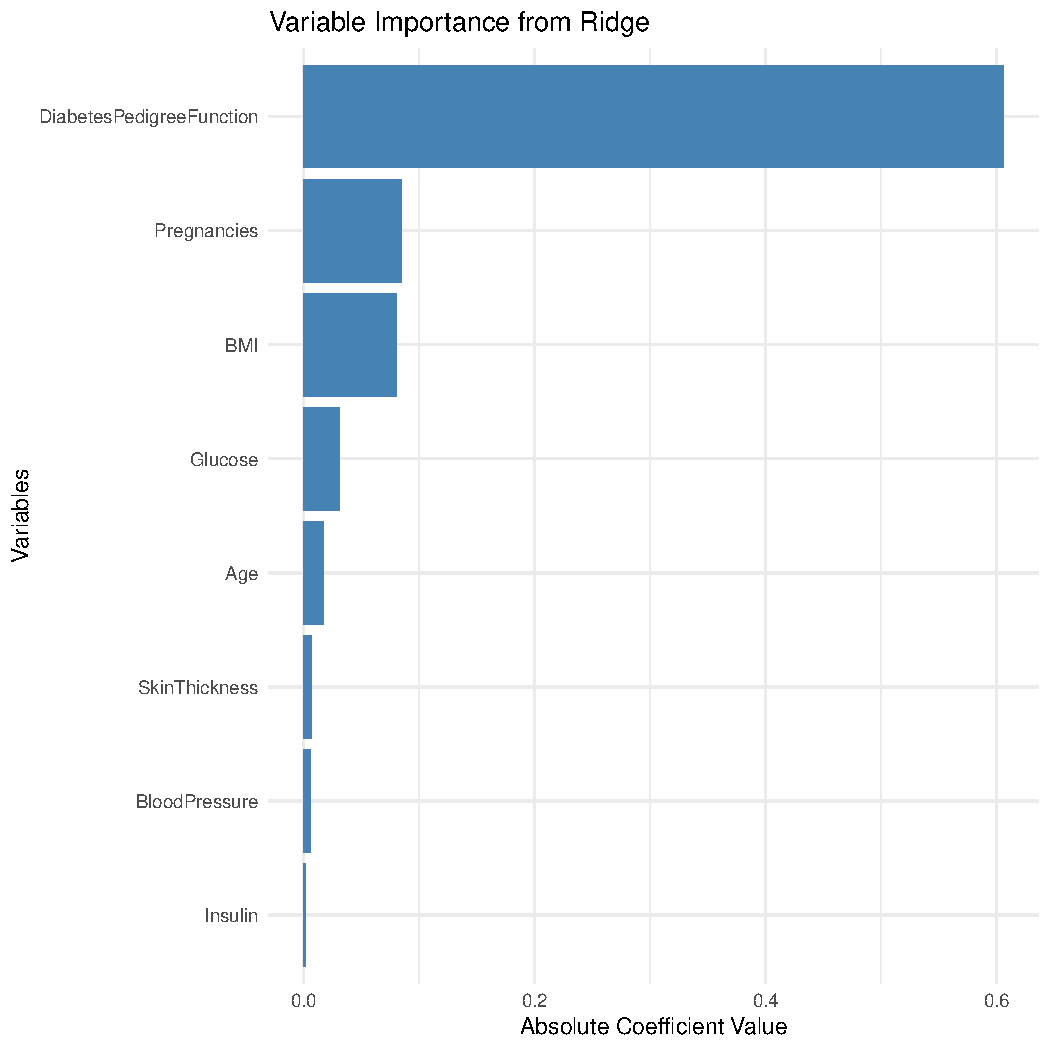
\includegraphics[width=0.7\columnwidth]{./Figures/logist/variable_importance_ridge.pdf}
\end{column}
\end{columns}

\end{frame}

\begin{frame}{ElasticNet and AdaLasso variable importance}

\vspace*{-1em}\begin{columns}[T]
\begin{column}{0.5\textwidth}
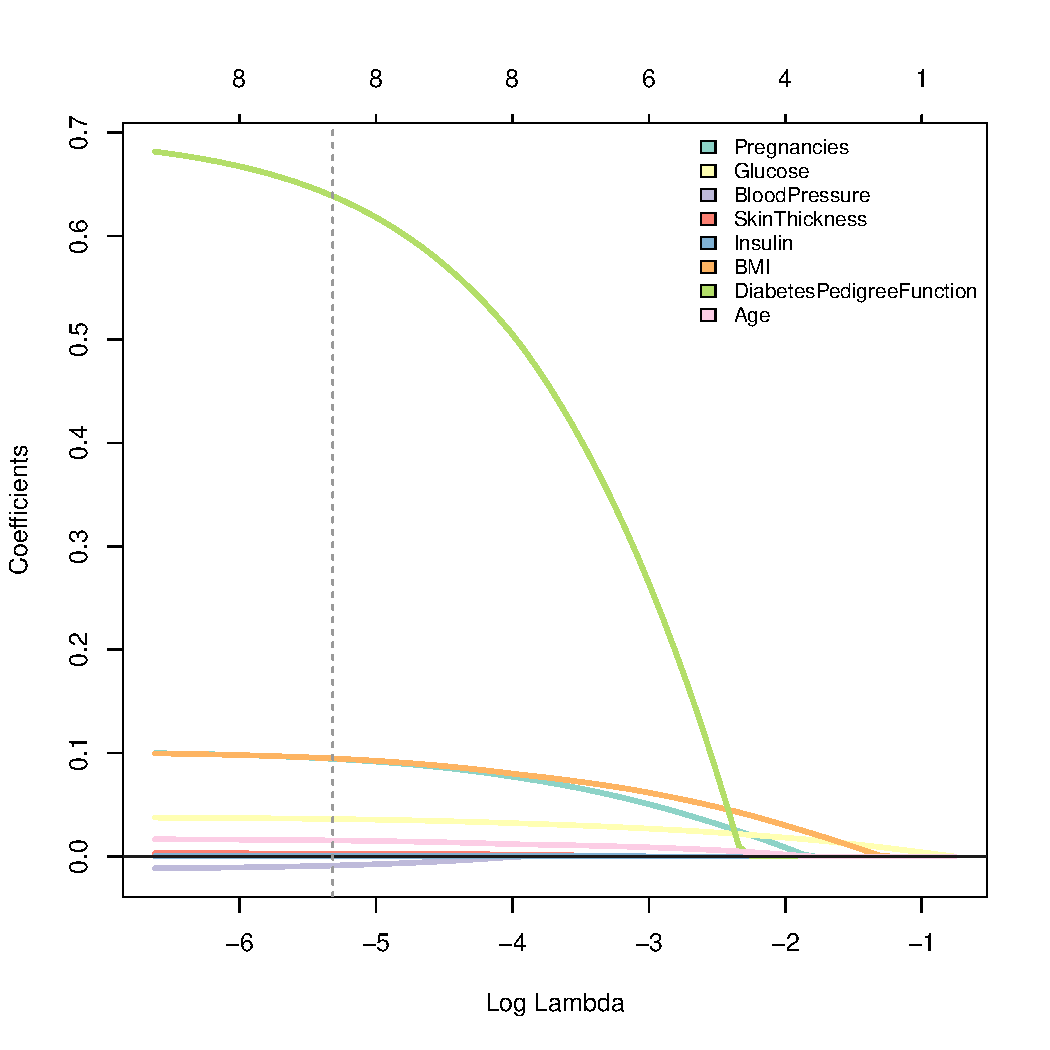
\includegraphics[width=0.85\columnwidth]{./Figures/logist/diabetes_elasticnet.pdf}
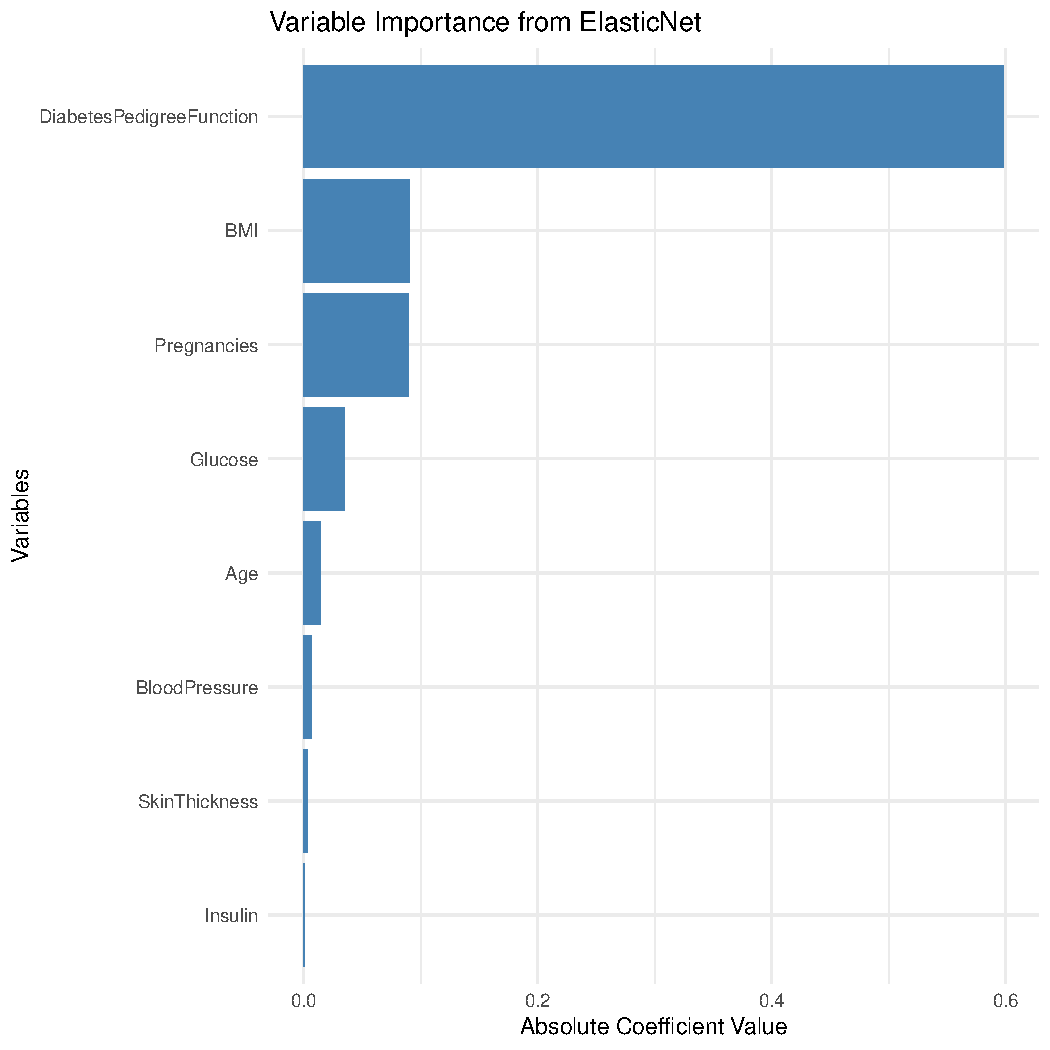
\includegraphics[width=0.7\columnwidth]{./Figures/logist/variable_importance_elasticnet.pdf}
\end{column}
\begin{column}{0.5\textwidth}
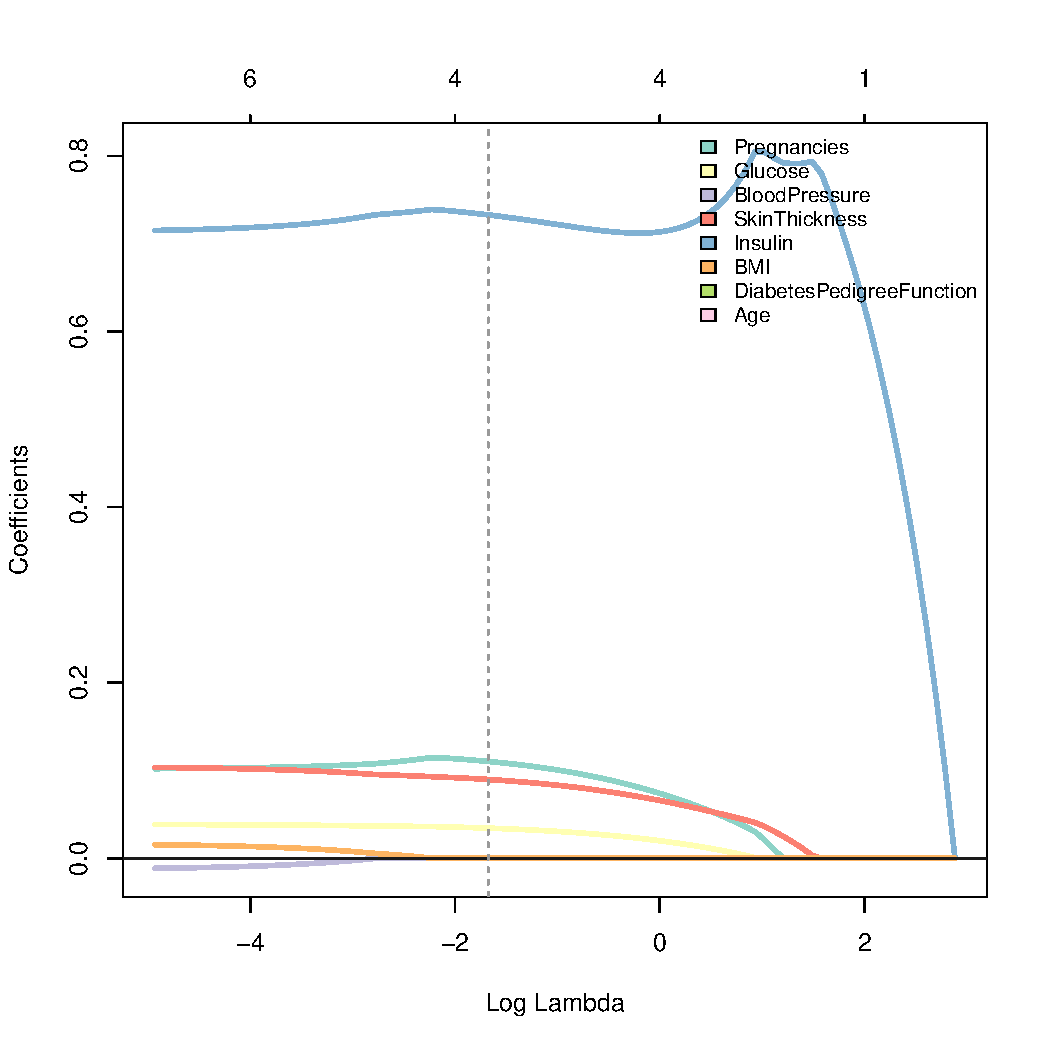
\includegraphics[width=0.85\columnwidth]{./Figures/logist/diabetes_adalasso.pdf}
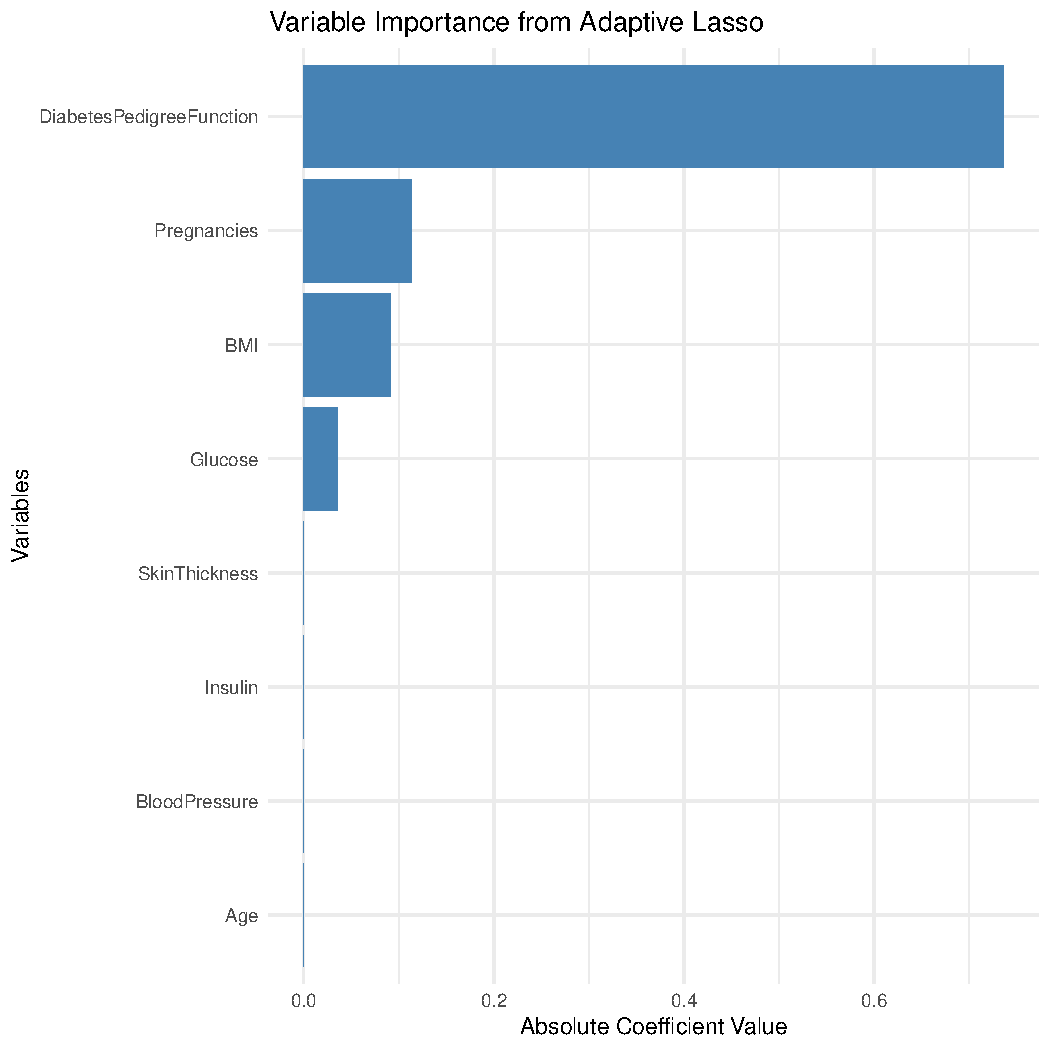
\includegraphics[width=0.7\columnwidth]{./Figures/logist/variable_importance_adalasso.pdf}
\end{column}
\end{columns}

\end{frame}

%\begin{frame}{Results}
%    \begin{table}
%\sisetup{round-mode=places}
%\resizebox{\textwidth}{!}{
%\begin{tabular}{lS[round-precision=4]S[round-precision=4]S[round-precision=4]}
%	Model & {Train score} & {Test score} & {\(\lambda\)} \\
%	\midrule
%	Lasso & 0.7714844 & 0.7695312 & 0.005678404 \\
%	Ridge & 0.7695312 & 0.765625 & 0.02346324  \\
%    ElasticNet & 0.7734375 & 0.7695312 & 0.008591009  \\
%    AdaLasso & 0.7714844 & 0.7695312 & 0.005678404 \\
%	\bottomrule
%\end{tabular}}
%\end{table}
%\end{frame}